\PassOptionsToPackage{unicode=true}{hyperref} % options for packages loaded elsewhere
\PassOptionsToPackage{hyphens}{url}
%
\documentclass[english,man]{apa6}
\usepackage{lmodern}
\usepackage{amssymb,amsmath}
\usepackage{ifxetex,ifluatex}
\usepackage{fixltx2e} % provides \textsubscript
\ifnum 0\ifxetex 1\fi\ifluatex 1\fi=0 % if pdftex
  \usepackage[T1]{fontenc}
  \usepackage[utf8]{inputenc}
  \usepackage{textcomp} % provides euro and other symbols
\else % if luatex or xelatex
  \usepackage{unicode-math}
  \defaultfontfeatures{Ligatures=TeX,Scale=MatchLowercase}
\fi
% use upquote if available, for straight quotes in verbatim environments
\IfFileExists{upquote.sty}{\usepackage{upquote}}{}
% use microtype if available
\IfFileExists{microtype.sty}{%
\usepackage[]{microtype}
\UseMicrotypeSet[protrusion]{basicmath} % disable protrusion for tt fonts
}{}
\IfFileExists{parskip.sty}{%
\usepackage{parskip}
}{% else
\setlength{\parindent}{0pt}
\setlength{\parskip}{6pt plus 2pt minus 1pt}
}
\usepackage{hyperref}
\hypersetup{
            pdftitle={Online Social Cohesion Reflects Real-World Group Action in Syria during the Arab Spring},
            pdfkeywords={social cohesion, recurrence quantification analysis, complex systems, Twitter, Arab Spring},
            pdfborder={0 0 0},
            breaklinks=true}
\urlstyle{same}  % don't use monospace font for urls
\usepackage{longtable,booktabs}
% Fix footnotes in tables (requires footnote package)
\IfFileExists{footnote.sty}{\usepackage{footnote}\makesavenoteenv{longtable}}{}
\usepackage{graphicx,grffile}
\makeatletter
\def\maxwidth{\ifdim\Gin@nat@width>\linewidth\linewidth\else\Gin@nat@width\fi}
\def\maxheight{\ifdim\Gin@nat@height>\textheight\textheight\else\Gin@nat@height\fi}
\makeatother
% Scale images if necessary, so that they will not overflow the page
% margins by default, and it is still possible to overwrite the defaults
% using explicit options in \includegraphics[width, height, ...]{}
\setkeys{Gin}{width=\maxwidth,height=\maxheight,keepaspectratio}
\setlength{\emergencystretch}{3em}  % prevent overfull lines
\providecommand{\tightlist}{%
  \setlength{\itemsep}{0pt}\setlength{\parskip}{0pt}}
\setcounter{secnumdepth}{0}

% set default figure placement to htbp
\makeatletter
\def\fps@figure{htbp}
\makeatother

% Manuscript styling
\usepackage{upgreek}
\captionsetup{font=singlespacing,justification=justified}

% Table formatting
\usepackage{longtable}
\usepackage{lscape}
% \usepackage[counterclockwise]{rotating}   % Landscape page setup for large tables
\usepackage{multirow}		% Table styling
\usepackage{tabularx}		% Control Column width
\usepackage[flushleft]{threeparttable}	% Allows for three part tables with a specified notes section
\usepackage{threeparttablex}            % Lets threeparttable work with longtable

% Create new environments so endfloat can handle them
% \newenvironment{ltable}
%   {\begin{landscape}\begin{center}\begin{threeparttable}}
%   {\end{threeparttable}\end{center}\end{landscape}}
\newenvironment{lltable}{\begin{landscape}\begin{center}\begin{ThreePartTable}}{\end{ThreePartTable}\end{center}\end{landscape}}

% Enables adjusting longtable caption width to table width
% Solution found at http://golatex.de/longtable-mit-caption-so-breit-wie-die-tabelle-t15767.html
\makeatletter
\newcommand\LastLTentrywidth{1em}
\newlength\longtablewidth
\setlength{\longtablewidth}{1in}
\newcommand{\getlongtablewidth}{\begingroup \ifcsname LT@\roman{LT@tables}\endcsname \global\longtablewidth=0pt \renewcommand{\LT@entry}[2]{\global\advance\longtablewidth by ##2\relax\gdef\LastLTentrywidth{##2}}\@nameuse{LT@\roman{LT@tables}} \fi \endgroup}

% \setlength{\parindent}{0.5in}
% \setlength{\parskip}{0pt plus 0pt minus 0pt}

% \usepackage{etoolbox}
\makeatletter
\patchcmd{\HyOrg@maketitle}
  {\section{\normalfont\normalsize\abstractname}}
  {\section*{\normalfont\normalsize\abstractname}}
  {}{\typeout{Failed to patch abstract.}}
\makeatother
\shorttitle{Arab Spring}
\author{[author names redacted for blind review]\\ Word count : 10981}
\affiliation{\phantom{a}}
\keywords{social cohesion, recurrence quantification analysis, complex systems, Twitter, Arab Spring}
\DeclareDelayedFloatFlavor{ThreePartTable}{table}
\DeclareDelayedFloatFlavor{lltable}{table}
\DeclareDelayedFloatFlavor*{longtable}{table}
\makeatletter
\renewcommand{\efloat@iwrite}[1]{\immediate\expandafter\protected@write\csname efloat@post#1\endcsname{}}
\makeatother
\usepackage{csquotes}
\usepackage{setspace}
\ifnum 0\ifxetex 1\fi\ifluatex 1\fi=0 % if pdftex
  \usepackage[shorthands=off,main=english]{babel}
\else
  % load polyglossia as late as possible as it *could* call bidi if RTL lang (e.g. Hebrew or Arabic)
  \usepackage{polyglossia}
  \setmainlanguage[]{english}
\fi

\title{Online Social Cohesion Reflects Real-World Group Action in Syria during the Arab Spring}

\date{}

\abstract{In recent years, political activists have taken to social media platforms to
rapidly reach broad audiences. Despite the prevalence of micro-blogging in
these sociopolitical movements, the degree to which virtual mobilization
reflects or drives real-world movements is unclear. Here, we explore the
dynamics of real-world events and Twitter social cohesion in Syria during the
Arab Spring. Using the nonlinear methods cross-recurrence quantification
analysis and windowed cross-recurrence quantification analysis, we investigate
if frequency of events of different intensities are coupled with social
cohesion found in Syrian tweets. Results indicate that virtual social cohesion
is coupled with the counts of all and negative events each day but shows a
more nuanced connection to positive events, suggesting that virtual
mobilization does reflect real-world movements. We conclude with a discussion
of implications and applications of nonlinear methods in political science
research.
}

\begin{document}
\maketitle

Before social media, people coordinated protests using phone tree calling sheets
and mimeographed flyers, through in-person meetings of social organizations and
churches, and by word of mouth. They gathered together and hand-made protest
signs that reflected their agendas. As McAdam found, people were more likely to
join movements when they had a personal connection (McAdam 1986; McAdam and Paulsen 1993): Historically, strong ties have been strong predictors of
involvement in high-risk protest activity.

The cohesiveness and strength of social movements before the Internet were
operationalized by the number of people present and through the political events
that precipitated and resulted from social gatherings \emph{en masse}. Cohesive
social movements were reflected in their cohesive placards and posters. For
example, the pervasive \enquote{I am a man} posters during the 1968 sanitation workers'
strike reflected their internal cohesion and unified, goal-oriented movement
(Windsor 2020).

However, the rise of the Internet and its decentralized online networks have
upended theories about recruitment to---and participation in---social movements.
Strong interpersonal ties have yielded to weak impersonal ties that strongly
predict involvement in social movements (Steinert-Threlkeld 2017). Measurements
of social movements have similarly evolved from ethnographic interviews to \enquote{big
data} analyses of social media.

Amid the cacophony of messages during political upheaval---such
as the Arab Spring---consistent themes emerge through hashtags, retweets, and
the repeated mentions of concepts such as regime, demonstration, and
human rights. The cohesiveness of these themes (i.e., whether movement
participants are metaphorically singing in one voice) reflects the real-world
events happening contemporaneously with collective action in social movements or
civil conflicts.

In the present research, we investigate the relationship between linguistic
cohesion and social cohesion in times of social conflict and unrest. We tackle a
question related to the one posed by Zeitzoff (2017): How does
social media reflect on-the-ground realities during times of social conflict? To
do so, we examine patterns of linguistic cohesion on Twitter and their
connection to real-world events during the Arab Spring uprising in Syria between
March and June 2012.

Disentangling the complicated relationship between mass online
mobilization---and social mobilization in person---continues to be relevant,
even as our modes of communication change. Accordingly, the political events
around the Arab Spring are still being understood. As Zeitzoff
(2017) recognizes, social media is changing conflict, but the
mechanisms and relationships by which it does so are still largely unknown.

\hypertarget{syria-in-context}{%
\subsection{Syria in Context}\label{syria-in-context}}

The decades preceding the Arab Spring in Syria were marked by repression and
fear. In 1971, Hafez al-Assad overthrew the previous leader and remained in
power for thirty years, presiding during regional contentiousness and
cooperation until his death in 2000. His son, Bashar al-Assad, continued the
regime of authoritarian leadership after assuming his office. The Assad lineage
hails from a minority Islamic sect (the Alawites) in a multi-religious and
multi-ethnic country comprising Christians, Sunni and Shia Muslims, Kurds, and
Palestinian refugees.

In December 2010, a Tunisian man named Mohamed Bouazizi was unjustifiably
stripped of his vendor cart by municipal officials. His humiliation led him to
set himself on fire in protest to the authoritarian rule, leading to his death
several days later. His actions served as a catalyst for the Tunisian
Revolution, and one week after his death, Zine El Abidine Ben Ali---the
longstanding authoritarian president---fled the country. The events of Tunisia
rapidly spread to surrounding countries also subject to unjust authoritarian
rule, including Egypt, Libya, and Syria.

Following a wave of democratization efforts across the Middle East and North
Africa, modest Syrian protests began in March 2011. The regime responded harshly
with imprisonments, detentions, censorship, and military operations as the
resistance to Assad's regime spread. The fighting escalated dramatically in
March 2012, after increased unrest in the western city of Homs. International
actors---including the Red Cross/Red Crescent Society, the United Nations
General Assembly, the U.N. Security Council, and individual world
leaders---worked toward cease-fires, negotiations, and concessions without much
success. While many high-level military and diplomatic officials defected,
numerous loyal forces continued the regime's repression, and the Syrian people
turned to social media to coordinate their activism and communicate to the
world. Between March and June 2012, more than 8 million tweets were sent within
Syria, revealing the details of the conflict suppressed by the government.

Syria is a multi-ethnic, multi-lingual, and multi-religious state. Kurdish
people make up between 10-15\% of the population, Alawites between 8-15\%, and
Christians about 10\%. There are also much smaller sects (e.g., Ismailis, Druze),
but Sunni Muslims comprise the vast majority of society. Most people speak
Arabic as their primary language. Most policy reports addressing the current
conflict report on the cohesion of the ruling Alawite military elite, rather
than on the cohesiveness of the opposition movement. However, the Sunni
majority's disaffection with the Syrian government and their lack of political
representation provide sufficient grievance and collective group identification
to make them a cohesive force.

\hypertarget{social-media-and-social-movements}{%
\subsection{Social Media and Social Movements}\label{social-media-and-social-movements}}

Massive online social cohesion can manifest in real-world social behavior.
Social media platforms enable online social cohesion by offering distributed
information-gathering and real-time information dissemination. Given its
accessibility and proficiency as an information exchange tool, Twitter has
provided social and political activists an opportunity to complement or even
replace real-world social mobilization. During the 2012 Italian protests for
global economic change, tweeting was determined to be more effective locally in
discussing real-world, real-time events than traditional mainstream media
platforms (Vicari 2013). As people increasingly rely on social media for
local news and information, we must understand exactly how these micro-blogs
connect to and reflect real-world action.

Along with Facebook, Twitter has been credited as essential to the Arab
Spring---both for protesters and for the government's response to them
(Comninos 2011). The Arab Spring has been deeply examined within the
political science literature (e.g., Lutterbeck 2013; Koehler 2017), but to our knowledge, the direct \emph{coupling} between
Syrian Twitter cohesion and international action has not been investigated. In
fact, some have been skeptical about the effect of social media on collective
action at all (Seay 2014).

This skepticism is summarized in a quote by Lisa Anderson (2011):

\begin{singlespace}
\setlength{\leftskip}{1cm}

\noindent The important story about the 2011
Arab revolts in Tunisia, Egypt, and Libya is not how the globalization of the
norms of civic engagement shaped the protesters' aspirations. Nor is it about
how activists used technology to share ideas and tactics. Instead, the critical
issue is how and why these ambitions and techniques resonated in their various
local contexts.

\setlength{\leftskip}{0pt}
\end{singlespace}

\noindent Others have similarly expressed hesitation about the role of online
organizing. Some have argued that real-life strong ties outweigh online weak
ties and that the power of the strong ties through in-person contact is critical
to recruiting people for higher-risk activities (Gladwell 2010; McAdam 1986).

Interestingly, these views may help make the case for bridging social media and
social mobilization. Such views suggest the strength of online social ties is
inextricably linked to the \emph{context} and \emph{ambitions} of the actors. Moreover,
research suggests that weak ties still retain considerable political power:
While strong ties tend to bind smaller groups, weak ties tend to bind groups
across distances (Granovetter 1973).

Social media generates critical information about events, including whether and
how a demonstration will take place, how many people participate, and how those
in power (e.g., state, military) respond. Similarly, these media platforms alert
us to more global shifts within a conflict, such as when fighting moves to a new
city or region, the number of casualties and wounded, and the types of weaponry
used by parties (Zeitzoff 2017). In monitoring social media channels,
government forces may respond to the perception that citizens are gaining
strength and sympathy. Governments have been shown to be quite tolerant of
dissent so long as it does not metamorphose into collective action
(King, Pan, and Roberts 2013).

Citizens communicate with each other with increased transparency due to the
ubiquitous availability of social media such as low-cost and egalitarian
platforms like Twitter. Citizens are able to access these tools via mobile
phones and computers with Internet connectivity, providing a stream of real-time
shared information. Citizens can share the location of events like protests and
military incursions, the degree of state repression, and the number of
casualties. In turn, the government---interested in remaining in
power---monitors social media platforms to ascertain emerging threats
(Comninos 2011), such as where new groups are forming, where existing
groups are strengthening, where gatherings are held, and who the leaders are.

An example of a leader expressing his interest in such public
conversation is given by Bashar al-Assad in a speech on June 3, 2012:

\begin{singlespace}
\setlength{\leftskip}{1cm}

\noindent I know that I have been away from the media for a long time, and I
have missed having direct contact with the citizens, but I have always been
following up with the daily occurrences and gathering the information so that my
speech can be built on what is said by the street.

\setlength{\leftskip}{0pt}
\end{singlespace}

\noindent With few exceptions, Assad chose to keep social media platforms up and
running. Gohdes (2015) notes that regimes can attempt to thwart
the growth of social protest online and in the streets by shutting down the
Internet. During these times, military repression increases, but government
information about the citizens decreases. As a result, regimes may elect to
maintain Internet connectivity to monitor and surveil their citizens.

At the same time, the insulation of online social platforms allows researchers
to detail real-world social dynamics at unprecedented resolution and scale
(Paxton and Griffiths 2017). The digital traces left by individuals and collectively as
groups are regarded as a valuable source of information that can offer powerful
insights into states of social disequilibrium, uprisings, and escalations into
civil wars. By examining these conversations, researchers can study the degree
of cohesion between speakers and the alignment between that cohesion and their
collective political behavior.

\hypertarget{the-role-of-cohesion-in-social-movements-and-civil-wars}{%
\subsection{The Role of Cohesion in Social Movements and Civil Wars}\label{the-role-of-cohesion-in-social-movements-and-civil-wars}}

People join social and political resistance movements because they feel a sense
of connection to the cause. Given that people are generally risk-averse,
overcoming inertia requires a strong connection to the group identity or a
strong aversion to an individual, event, or political injustice
(Goldstone 1980, 2011). Political resistance offers participants the
opportunity to \enquote{lose themselves} and relinquish their individual identity in
favor of identification with a larger group, contributing to a cohesive group
ready and mobilized for action (Hoffer 2011).

The type of collective contentious behavior that manifests in society is a
function of the available political opportunity structures. The political
opportunity structure is \enquote{comprised of \emph{(sic)} specific configurations of
resources, institutional arrangements and historical precedents for social
mobilization, which facilitate the development of protest movements in some
instances and constrain them in others} (Kitschelt 1986). What emerges
as strategies and tactics in contentious politics are a function of
what the system makes possible. This includes the number of people and their
disposition (i.e.~nonviolent or violent), as well as their internal structure.
The more cohesive a group is, the greater threat they pose to the establishment.

Cohesion is a familiar concept in the study of civil conflicts, as it pertains
to group affiliation and the ability to overcome collective action problems.
Individuals must act in concert---that is, cohesively---to accomplish the task
of challenging state authority (Olson 1965; Eisinger 1973; Tilly 2004; Francisco 1995).
Viewing rebel recruitment during civil conflicts as a function of internal
cohesion, rebel movement success is influenced by the degree of group cohesion,
which itself is a function of geographic distance, ideology, and ethnicity
(Gates 2002). Within Syria, multiple rebel groups exist, sourcing
fighters locally (from the disaffected Syrian population) and internationally
(from transnational terrorist organizations). Groups compete intensely with one
another for recruitment in the rebel movement and often punish defectors for
nonparticipation (Gates 2002).

Another factor influencing social cohesion during social movements and civil
wars is ethnic identity and the degree of ethnic conflict associated with the
movement. Greater degrees of ethnic conflict increase the salience of ethnic
identity, leading people to identify more strongly with their own ethnic
identity (Sambanis and Schulhofer-Wohl 2009). As ethnic conflict intensifies, groups seek to become
more quintessentially like the typical member of their ethnic group. This can
manifest in a number of ways, including in behavior on social media. However,
this may also include a general identification across ethnic groups in a
membership of an opposition to an oppressive leader.

The civil war literature has also explored the role of social cohesion. Social
homogeneity increases the likelihood of social conflict, especially when the
society is polarized (Collier and Hoeffler 2004); this is partly due to nationalist
groups' strong identification with a collective identity (Cederman and Girardin 2007)
and their social solidarity (Sambanis and Schulhofer-Wohl 2009). These same processes can be
similarly important for rebels (Anyanwu 2002). Referencing Gurr's
(2000) work on minorities at risk, Regan and Norton
(2005) note that

\begin{singlespace}
\setlength{\leftskip}{1cm}

\noindent a religious or linguistic minority
might suffer disproportionately in a given society, and this form of
aggrievement can lead to unrest across the social lines that distinguish the
minority group. Therefore, while collective cohesion is a function of targeted
maldistributions, it is individual penury that allows for this collective
mobilization.

\setlength{\leftskip}{0pt}
\end{singlespace}

The body of previous work concurs that group cohesion matters to group
mobilization. We build on this by providing a quantitative approach to
understanding cohesion from multiple levels and by incorporating analytic tools
that allow us to investigate the interconnectedness of those levels.

\hypertarget{cohesion-a-multi-leveled-multi-layered-concept}{%
\subsection{Cohesion: A Multi-Leveled, Multi-Layered Concept}\label{cohesion-a-multi-leveled-multi-layered-concept}}

We contextualize linguistic cohesion with social mobilization and response to
the relative intensity of the conflict. Cohesion is a multi-layered concept
referring to the connectedness of speakers, actions, and societies. It
reflects the continuity of language and expression and shows the
connectivity of participants in a social movement. To address the relationship
between language and discourse and social movements, we adopt an
interdisciplinary approach that incorporates linguistics, psychology, and
political science using nonlinear dynamical systems methodology to disentangle the
relationship between language and action.

\hypertarget{lexical-and-interlocutor-cohesion}{%
\subsubsection{Lexical and Interlocutor Cohesion}\label{lexical-and-interlocutor-cohesion}}

Just as real-world social cohesion can be quantified, so can online cohesion.
One kind of cohesion is the similarity in language use on social
media. This implicit or explicit similarity can indicate shared
beliefs, thoughts, and feelings, as has been studied in research on language
style in psycholinguistics and social psychology (Gonzales, Hancock, and Pennebaker 2010; Tausczik and Pennebaker 2010; Brennan and Clark 1996). Although previous work on language style has often
focused on individuals and small groups, this can be scaled up to examine
massive social-level changes (Michel et al. 2011; Fusaroli et al. 2015).

The first level of cohesion that we will consider are the words within social
media posts. In Figure \ref{fig:cohesion-in-tweets}, we see four sequential
tweets of four words each. Each sequential tweet contains some content
included in the previous tweets. The linguistic construct of content word
overlap measures the relationship across units of meaning---here, tweets---where
identical and semantically similar words are repeated (Graesser et al. 2004). These
repeated lexical items constitute a theme; on Twitter, this might be a
particular hashtag, a name, a location, or another nominal category. This
localized cohesion is referential; words are repeated and co-referred across
tweets, creating a sense of continuity and cohesiveness.

Typically, these analyses focus on \emph{content words} (e.g., nouns, adjectives,
verbs), which convey more meaningful semantic information than \emph{function words}
(e.g., articles, conjunctions). While function words can provide important
information about complexity and language structure
(Tausczik and Pennebaker 2010), content words have more specialized meaning and
are therefore more useful when researchers want to understand \emph{what} people are
discussing, rather than \emph{how} they are discussing it (Graesser et al. 2004; McNamara et al. 2014).

In estimating cohesion in Twitter posts, tweets that share content words
yield higher cohesion values, even among speakers with opposing
views on the subject matter. Repetition of terms and concepts is captured by
reiteration, which is a type of lexical cohesion in which a subsequent item
repeats a previous item, or refers to it through synonymous language
(Halliday and Hasan 1976). In social media, we can conceive of retweets (i.e., reposts
or forwards of previous messages) as a form of reiteration
that increase message cohesion. Since retweets replicate verbatim some part of
another tweet, these tweets would also have higher cohesion. Hashtags function
similarly and are included in our analysis.

\begin{figure}
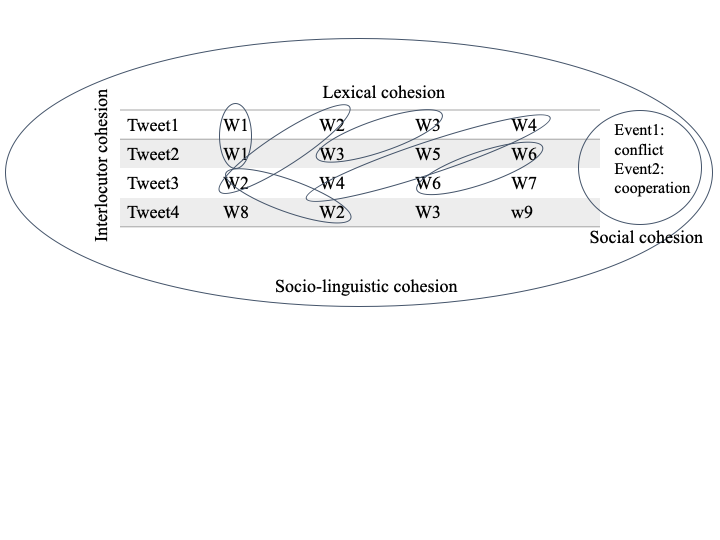
\includegraphics[width=1\linewidth]{./figs/cohesion-in-tweets} \caption{A visual representation of cohesion in tweets. The shared content words--either identical or semantically similar--constitute a theme around which cohesion is occuring.}\label{fig:cohesion-in-tweets}
\end{figure}

The use of similar language can provide insight into \emph{interlocutor cohesion}, or
the degree to which people are talking about similar things. This can include
people who are talking about similar things from radically perspectives, as well
as those who are talking about something from the same perspective. Previous
research from political science has investigated these ideas (Windsor 2020): The
\enquote{Occupy Wall Street} movement has been held up as an example of a movement with
low interlocutor and linguistic cohesion because of its wide range of signs and
slogans, while the \enquote{I am a man} protest (during the 1968 sanitation workers'
strike in Memphis, TN) or the \enquote{Black Lives Matter} placards (following the
uprising in Ferguson, MO) have high lexical and interlocutor cohesion
(Edgar and Johnson 2018).

Fed by lexical cohesion, interlocutor cohesion ebbs and flows, contextualized by
changing real world events. Interlocutor cohesion may increase preceding an
in-person social mobilization event, alerting a repressive government that
collective mobilization is happening. Interlocutor cohesion may also respond to
exogenous events such as spontaneous, unprovoked militarized conflict.

Given the importance of lexical and interlocutor cohesion for messaging in
political movements, lexical cohesion may be important trace data for
researchers interested in leveraging social media data to analyze social
movements. Similar to large-scale studies of sociocultural movements (sometimes
referred to as \emph{culturomics}; e.g., Michel et al. 2011), political
scientists can track the ways in which conversations on social media coalesce or
diffuse around similar content words. In this way, it matters relatively little
whether the interlocutors have precisely the same views: The point is to
understand whether the society-level conversation is converging on similar
themes.

\hypertarget{social-and-political-cohesion}{%
\subsubsection{Social and Political Cohesion}\label{social-and-political-cohesion}}

Real-world collective action is known to bring about a sense of togetherness,
also known as \enquote{collective effervescence} (Durkheim 1995). This feeling
of being a part of something larger than oneself leads individuals to act in
ways that would not have on their own. Being overcome with this feeling can lead
to violence (Collins 2009; Spaaij 2014). Conversely, increased
exposure to violence can result in positive social cohesion. Gilligan, Pasquale, and Samii (2014)
found that exposure to fatal wartime violence resulted in increased prosocial
motivations, including cooperative behaviors, feelings of trust, and overall
community-level social cohesion.

At the same time, behavioral similarity in certain contexts has been
connected to important psychological and social effects. For example, shared
language is associated with rapport (both in face-to-face and computer-mediated
conversations; Niederhoffer and Pennebaker 2002; Riordan et al. 2011) and
can even be connected to better performance on shared tasks (as long as
the language is relevant to the task at hand; Fusaroli et al. 2012). Shared
movement is associated with greater group bonding and greater willingness
to contribute to the group (Wiltermuth and Heath 2009), and shared identity
leads to a greater willingness to adopt the group's goals and
motivations (Walton et al. 2012).

We expect to see increased linguistic cohesion among people participating in
online discussions about an idea, event, individual, or movement. Given that
Syrian protesters coordinated their activity through Twitter by discussing their
own events (e.g., planned protests, active demonstrations) and their reactions
to events happening around them (e.g., government reactions, international
action or inaction), the cohesion in social media should correlate with the
social cohesion of the group (Zeitzoff 2011).

Political and social cohesion in the world can be modeled using event data which
encodes who does what to whom on a given day. CAMEO (Conflict and Mediation
Event Observations) encode a set of activities with numerical values, rescaled
to reflect a conflict-cooperation scale (Schrodt and Hall 2006; Goldstein 1992). These event codes include a range of behaviors, from
making public statements and appeals, to demanding, threatening, protesting, and
using unconventional mass violence.

Social cohesion can have real and wide-ranging impacts on a political movement
and the people in it. A socially cohesive group is inherently more threatening
to the existing regime because it reflects momentum in collective opposition and
the professionalization of alternate leadership. Global insurgency movements
exhibit similar patterns in their social structure (Bohorquez et al. 2009).
Rather than patchwork messages via Twitter, emergent or intentional cohesive
online messaging---using similar language, paralleling in-person messaging
(Windsor 2020)---demonstrates increased organizational structure, inciting a
government response.

Thus, lexical and interpersonal cohesion are hypothesized to be tied to social
and political cohesion. Shared online language may lead to the development or
expression of shared identity (Wiltermuth and Heath 2009). This, in turn, may
drive individuals' propensity to engage in coordinated behavior for the group
(Wiltermuth and Heath 2009; Walton et al. 2012). Taken together, these processes may
increase movement participants' weak and strong ties (Granovetter 1973; Gladwell 2010; McAdam 1986), building the movement by expanding and deepening
heterogenous ties. Therefore, during social conflict, the linguistic cohesion
of the online conversation should correspond to the degree of social cohesion on
the ground.

Steinert-Threlkeld (2017) modeled a similar relationship
between social media and social mobilization alongside event data. That
groundbreaking work demonstrated that participants on the fringe of a social
movement contribute substantially to the overall level of protest. Here, in
addition to providing new methods to this area, we build on this work by
demonstrating how sociolinguistic cohesion evolves in tandem with negative and
positive exogenous events.

\hypertarget{sociolinguistic-cohesion-connectedness-of-speakers-ideas-and-events}{%
\subsubsection{Sociolinguistic Cohesion: Connectedness of Speakers, Ideas, and Events}\label{sociolinguistic-cohesion-connectedness-of-speakers-ideas-and-events}}

We tie the constructs of lexical, interlocutor, and social cohesion together in
a theoretical framework called \emph{sociolinguistic cohesion}, as shown in Figure
\ref{fig:theoretical-framework}. Previous values of linguistic cohesion should
influence future values of linguistic cohesion and future actions in the real
world space. Previous events influence future events and future linguistic
cohesion in social media.

Sociolinguistic cohesion is not a static concept. Just as social movements
experience increased participation and setbacks---indicating dynamic
relationships among participants and between participants and the sociopolitical
environment---sociolinguistic cohesion is also dynamic, reflecting the changing
states of the political sphere. Other scholars have noted the diffusion of
messages that reach critical mass, allowing for \enquote{behaviors, beliefs, and
preferences} to spread within a population (Barash, Cameron, and Macy 2012). Cohesion
changes over time in response to external events and the internal dynamics of
the social movement, even if the social interaction occurs entirely
online (Centola and Macy 2007).

Lexical cohesion, then, is a useful indicator of social cohesion in political
crisis. Lexical cohesion happens at the word level. Interlocutor cohesion
happens between speakers. Political cohesion happens at the social level during
moments of political crisis, like civil wars and social movements.
Sociolinguistic cohesion comprises lexical, interlocutor, and sociopolitical
events, in which the words and their context reveal the disposition of socially
connected linguistic communities. It accounts for the cohesion between multiple
speakers in an environment as their language becomes more similar.
Sociolinguistic cohesion also addresses how groups involved in political
rebellion converge to mount sustained resistance to state authority.

Related previous work has also explored diffusion of hashtags in viral contagion in
Nigeria, a phenomenon similar to what we identify as sociolinguistic cohesion
(Fink et al. 2016). The prevalence and rate of particular hashtags were
contributed to the overall sociolinguistic cohesion. The more that people
reuse hashtags or common phrases, the greater the sociolinguistic cohesion when
this phenomenon occurs during socially significant times like protests
(State and Adamic 2015).

Combining these separate threads, it is reasonable to expect that real-world
actions and online social interactions would be enmeshed, driving and being
driven by one another. From a dynamical systems perspective, online social
cohesion and in-person action can be considered two complementary components of
a single system, mutually constrained and constantly interacting and influencing
one another (Mahner and Bunge 1997). Investigation of the coupling of
real-world mobilization and social cohesion could provide new insight into the
power of social media during mobilization and the ways in which individuals
utilize it to bring about, or respond to, social change. Increasingly, social
media platforms are being utilized during social mobilization
(McAdam, Tarrow, and Tilly 2003; Koopmans 2004), but the relationship between virtual and real-world
mobilization is still largely unknown. The present work aims to understand how
physical and virtual movements coexist and interact from a dynamical systems
perspective.

\begin{figure}
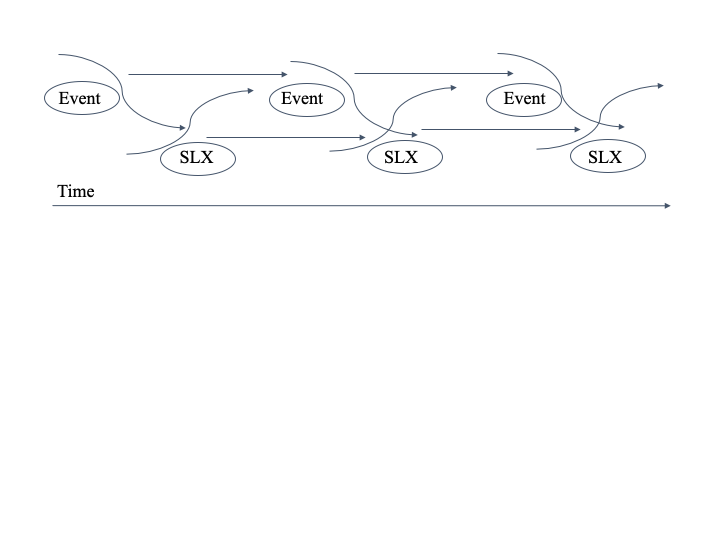
\includegraphics[width=1\linewidth]{./figs/theoretical-framework} \caption{The theoretical framework for sociolinguistic cohesion. Real-world events and linguistic cohesion continually interact and influence one another throughout time.}\label{fig:theoretical-framework}
\end{figure}

\hypertarget{using-nonlinear-methods-to-capture-complex-relationships}{%
\subsection{Using Nonlinear Methods to Capture Complex Relationships}\label{using-nonlinear-methods-to-capture-complex-relationships}}

Given the hypothesized interrelationship between the real-world and online
actions---and the notorious messiness of naturally occurring data---it is
critical to find appropriate analysis tools that can identify the complex
interconnections. Traditional linear analyses have led to many notable
discoveries in the domains of psychology and political science, but time series
data pose problems that are not easily overcome with these methods. Events have
historically been conceptualized as linear chains of smaller, sequential events
with one occurrence leading to the next. Certain kinds of data are relatively
well-suited to these analyses, but messy, complex, variable data from real-world
events can pose challenges, from overpowered samples to violation of underlying
statistical assumptions (Paxton and Griffiths 2017).

At the same time, the foundational theoretical assumptions of a linear world has
been increasingly replaced by ideas from dynamical systems theory. Rather than a
chain of events, time series data can be thought of as nested occurrences, where
mutually constrained parts (e.g., citizens, governments, real-world events,
social media platforms) are constantly interacting, leading to more global
behaviors that are larger than the sum of the parts (Turvey 2018). When
analyzed as dynamical systems, many phenomena exhibit new nonlinear patterns
that were formerly overlooked. Nonlinear methods provide means for capturing the
rich temporal dynamics and variability that unfold in time series data.

Although a number of other nonlinear methods exist, the primary nonlinear methods
used in the current work are cross-recurrence quantification analysis (CRQA; Zbilut, Giuliani, and Webber Jr 1998) and its offshoot, windowed cross-recurrence quantification
analysis (WCRQA; Webber Jr and Zbilut 2005). CRQA has successfully been used to gain
a better understanding of many complex human phenomena, including a variety of
human social interactions (for a review, see Fusaroli, Konvalinka, and Wallot 2014). Much as it
has for psychology, we argue that the use of nonlinear methods in the
investigation of political science phenomena will lead to new insights and the
development of more robust theories.

\hypertarget{the-present-work}{%
\subsection{The Present Work}\label{the-present-work}}

Social media has become a primary platform for social movements and activism
across the world, but the extent to which virtual activism reflects and drives
real-world mobilization is still largely unknown. In the current work, we
conceptualize the physical and virtual movements as a dynamical system, both
constantly interacting and influencing the other. We aim to study this by
analyzing the real-world events and online social cohesion during nearly three
months of the Arab Spring. Both real- and virtual-world collective coordination
were powerful tools in the events of the Arab Spring and are undeniably linked.
This study aims to explore the dynamics of Twitter users in Syria, who used the
social media platform to raise awareness about the Arab Spring and bring about
mass mobilization.

Using cross-recurrence quantification analysis (CRQA; Zbilut, Giuliani, and Webber Jr 1998) and
windowed cross-recurrence quantification analysis (WCRQA; Webber Jr and Zbilut 2005), we analyzed the co-evolution of social cohesion online
and real-world events. Specifically, using heterogeneous data from March 30,
2012, to June 15, 2012, we compared the social cohesion of Syrian tweets with
the counts of all, positive, and negative real-world events derived from
international event data (i.e., the Integrated Crisis Early Warning System; Boschee et al. 2015).

We hypothesized that the count of all events and the count of negative events
would show high levels of determinism, as this time period was marked by daily
violence which often leads to increased salience. We also hypothesized that the
count of positive events would not show patterns of determinism, as these events
were likely overshadowed by the salient negative daily occurrences. After
testing these hypotheses, we then conducted exploratory analyses to further
examine the patterns identified with CRQA. Using WCRQA, we sought to identify
shifts in the dynamics of the systems that could then be linked to real-world
shifts in conflict frequency. Through these analyses, our two primary goals in
the current work were to uncover (1) how different intensities during times of
turmoil may enhance or deter social cohesion in social media communication and
(2) how social mobilization may be evident in the dynamic coupling of cohesion
and real-world events.

An additional focus of the current work is to introduce cross-recurrence
quantification analysis---a longstanding method from physics that has since
become influential in a variety of other fields---to political science. We do so
by providing detailed descriptions of the methods and providing clear directions
about interpretation and significance testing even with relatively small-\emph{n} or
case studies. After demonstrating these methods' utility with this dataset, we
close the paper with specific suggestions to political scientists interested in
these methods.

This work is a reproducible manuscript. All code and analyses can be found at:
{[}redacted for blind review{]}.

\hypertarget{method}{%
\section{Method}\label{method}}

\hypertarget{materials}{%
\subsection{Materials}\label{materials}}

\hypertarget{tweet-corpus}{%
\subsubsection{Tweet Corpus}\label{tweet-corpus}}

The corpus of tweets used included 0 Syrian tweets
occurring between March 30--June 15, 2012. Using the Twitter streaming API,
servers at the University of Texas at Austin collected the tweets. The servers
were run on a stable (LTS) version of Ubuntu Linus (v. 10.04) and were connected
directly to the high-bandwidth UT network maintained by IT services.

Tweets collected contained one or more of the following keywords: \enquote{syria,}
\enquote{syrian,} \enquote{damascus,} \enquote{homs,} \enquote{al-assad,} and \enquote{sunni.} These keywords were
chosen based on the most distinctive terms used in news articles covering the
Arab Spring in Syria at the time. A node.js script was used to reinitialize the
connection to Twitter's servers whenever the script timed out due to a period of
silence. The script requested data from the API endpoint using basic HTTP
authentication (OAuth was optional, at the time) at
\url{https://stream.twitter.com/1.1/statuses/filter.json}, and stored the data
directly to the local hard disk. The tweets were then post-processed with a
Python script to convert the JSON-formatted tweets to tab-separated files, which
were then compressed to maximize storage efficiency.

All scripts used for scraping tweets and compressing data can be found at
\url{https://github.com/chbrown/twilight}.

\hypertarget{event-data}{%
\subsubsection{Event Data}\label{event-data}}

Event data were obtained from the 2012 Integrated Crisis Early Warning System
(ICEWS; Boschee et al. 2015). The event data were first filtered to remove
incomplete and incorrectly formatted data. They were then filtered to include
only events that were directed at (i.e., \texttt{target}) Syria (\(n = 6300\)). To
explore the impact of outwardly directed Syrian events, the data were filtered
again to include events that were both directed at (i.e., \texttt{target}) or directed
by (i.e., \texttt{source}) Syria (\(n = 7990\)).

\hypertarget{data-preparation}{%
\subsection{Data Preparation}\label{data-preparation}}

\hypertarget{social-cohesion-metric}{%
\subsubsection{Social Cohesion Metric}\label{social-cohesion-metric}}

The social cohesion or linguistic similarity of daily tweets was calculated by
quantifying the frequency of shared content words with respect to those words'
frequencies in the entire tweet corpus. If a linguistic term has a high
frequency in one tweet but has a low frequency in the whole tweet corpus, then
it is more likely a content word and is thus given more weight in calculating
social cohesion. This method is similar to \emph{term frequency-inverse document
frequency} (tf-idf; see also Jones 1972; Robertson 2004).

The tweets were first sorted into ascending order by timestamp. They were then
grouped into successive sets of five tweets. Inverse frequency weighting for the
overlap words and all words was conducted for each pair of two tweets in the
group of five, then divided to get the social cohesion score for that pair (see
Eq. 1-3). This resulted in ten social cohesion values for each group of five
tweets; these values were then averaged to get a social cohesion score for the
entire set of five tweets. Finally, the mean of all average cohesion values for
all groups was taken to get a social cohesion score for each day.

\begin{align}
\text{Inverse frequency weighting of overlap words = }\sum_{i=1}^k
\frac{log(f(t_i, d1) + f(t_i, d2) + 1)}{log(f(t_i) + 1)}
\end{align}

\begin{align}
\text{Inverse frequency weighting of all words = }\sum_{i=1}^n \frac{log(f(t_i,
d1) + f(t_i, d2) + 1)}{log(f(t_i) + 1)}
\end{align}

\begin{align}
\text{Two tweets' similarity =}\frac{\text{inverse frequency weighting of overlap
words}}{\text{inverse frequency weighting of all words}}
\end{align}

\noindent The social cohesion calculation was performed on the tweet corpus
containing both English and Arabic tweets. All hashtags and URLs were included
in the analysis. The raw social cohesion time series can be seen in Figure
\ref{fig:raw-cohesion-ts}.

\begin{figure}
\includegraphics[width=6.5in]{./results/primary/raw-cohesion-ts} \caption{Raw social cohesion metric time series.}\label{fig:raw-cohesion-ts}
\end{figure}

\hypertarget{icews-event-time-series}{%
\subsubsection{ICEWS Event Time Series}\label{icews-event-time-series}}

Using the Integrated Crisis Early Warning System (ICEWS) developed at the
Defense Advanced Research Project Agency, the daily events were scored with an
intensity rating ranging from -10 to 10. Negative events---such as riots and
attacks---are coded with low negative numbers, while positive or peaceful events
are coded with high positive numbers. This well-validated coding scheme allows
for numerical quantification of different event types.

For both the target-only and the target and source data described above, time
series of the count of all events were generated by summing the total number of
events on each day, irrespective of ICEWS score. Similarly, time series of count
of positive events were generated by summing the number of ICEWS events for each
day that had an intensity rating greater than zero. Lastly, time series of count
of negative events were generated by summing the number of ICEWS events for each
day that had an intensity rating less than zero.

The raw event time series for target filtered data can be seen in Figure
\ref{fig:raw-event-ts-target}. The raw event time series for source and target
filtered data can be seen in Figure \ref{fig:raw-event-ts-source-target}.

\begin{figure}
\includegraphics[width=6.5in]{./results/primary/raw-event-ts-target} \caption{Raw event count time series for target filtered data.}\label{fig:raw-event-ts-target}
\end{figure}

\begin{figure}
\includegraphics[width=6.5in]{./results/primary/raw-event-ts-source-target} \caption{Raw event count time series for source and target filtered data.}\label{fig:raw-event-ts-source-target}
\end{figure}

\hypertarget{analyses}{%
\subsection{Analyses}\label{analyses}}

\hypertarget{cross-recurrence-quantification-analysis}{%
\subsubsection{Cross-Recurrence Quantification Analysis}\label{cross-recurrence-quantification-analysis}}

We first used cross-recurrence quantification analysis (CRQA; Zbilut, Giuliani, and Webber Jr 1998) to investigate the temporal patterns of social cohesion
and real-world events in Syria during Arab Spring. CRQA is an extension of RQA,
which captures the patterns of revisited states of a single time series
(Zbilut and Webber Jr 1992; Webber Jr and Zbilut 1994). CRQA allows for two time series
to be projected onto one another to investigate shared states and trajectories.
In CRQA, we track these shared states by identifying \emph{recurrent points}, or
intersections of time during which two signals shared or revisited the same
state. These shared states can be at the same time or at later points in the
time series. We can further chart shared trajectories by examining the
occurrences and patterns of multiple sequential recurrent points.

To perform CRQA, the time series must be converted to the same scale, while
still preserving a sampling rate that respects the native timescale of the
system (cf.~Nyquist frequency in signal processing; Grenander 1959).
Because the social cohesion and event data have different scales and values, we
converted each time series (e.g., Figure \ref{fig:raw-ts}) into deciles (e.g.,
Figure \ref{fig:deciled-ts}) to analyze the relative dynamics of different
levels of social cohesion and counts of all, positive, and negative events on
each day. We implemented CRQA using the \texttt{crqa} package (Coco and Dale 2018) for R
(R Core Team 2019).

\hypertarget{visualization}{%
\paragraph{Visualization}\label{visualization}}

A cross-recurrence plot (CRP) is the visual representation of CRQA. To construct
a cross-recurrence plot, two time series are plotted against each other on the
\(x\) and \(y\) axes. At every point where they share the same state, a point in
placed on the plot to indicate recurrence. (For categorical CRQA, this process
is similar to the Cartesian product.)

We can visually analyze these plots to reveal patterns of structure and
recurrence. The line \(y = x\) is known as the \emph{line of identity}. This line falls
where the time series match temporally. A filled line would indicate perfect
in-phase synchrony between the two time series. See Figures
\ref{fig:plot-rp-targ}-\ref{fig:plot-rp-source-targ} for examples of
RPs.

\hypertarget{metrics}{%
\paragraph{Metrics}\label{metrics}}

While visual inspections can be informative, we can derive a variety of
quantitative metrics from the cross-recurrence plot. Each of these metrics
provides information into the patterns and dynamics of the new shared system.
These metrics are also critical for inferential statistics. We will focus most
directly on two of these metrics: \emph{recurrence rate} and \emph{determinism}.

The percentage of recurrent points to total possible points is a metric called
the \emph{recurrence rate} (\emph{RR}). This metrics gives a general description of how
frequently the time series are sharing the same states. In the current study, a
recurrent point would indicate that the level of social cohesion and frequency
of events were at the same intensity.

Recurrent points that occur in successive moments form line structures. These
are conceptualized as shared trajectories, where the two time series are moving
together across time in a shared state. The percentage of recurrent points on
the plot that fall along diagonal line structures (i.e., two or more consecutive
points) is a metric called \emph{percent determinism} (or simply \emph{determinism};
\emph{DET}). For the current project, a high DET would indicate that not only are the
levels of social cohesion and frequency of events occurring at similar
intensities, but they are doing so across consecutive days.

A number of other metrics provide insight not only into the amount of structure
between the systems but about the nature of this shared structure. The average
length of the line structures is called \emph{mean line} (L), which can be
conceptualized as the average amount of time that the two time series move
together before one or both shift states. The longest line length is called \emph{max
line} (\emph{maxL}); it indicates the longest instance of being \enquote{stuck} in a
particular state together and is a measure of the stability of the system. The
total \emph{number of lines} on the plot (\emph{NRLINE}) scales with structure: The more
lines that exist, the more coupled the two systems are. The complexity or
variability of line lengths is captured by a metric called \emph{entropy}
(\emph{ENTR})---which may also be normalized by the total number of lines (i.e.,
\emph{normalized entropy}; \emph{rENTR})---and indicates the stability and predictability
of the system. When one of the signals gets \enquote{stuck} in a state and the other
moves on to other states, this results in vertical line structures, which are
quantified in \emph{laminarity} (\emph{LAM}; i.e., the proportion of points forming
vertical line structures) and \emph{trapping time} (\emph{TT}; i.e., the average length of
the vertical trajectories). For more detail on CRQA metrics, see Coco and Dale (2018).

\hypertarget{parameters}{%
\paragraph{Parameters}\label{parameters}}

To conduct the analyses on the decile data, the parameters were set to those
typically used in categorical CRQA: Delay was set to \(0\), embedding dimension
was set to \(1\), and radius was set to \(.001\) to allow for only exact recurrent
matches. No normalization was done, and lines were considered two or more
consecutive recurrent points. The Theiler window was set to \(0\) to include
points along the line of identity. For more details on the CRQA parameters and
how they impact the analysis, see Coco and Dale (2018).

\hypertarget{permutation-test}{%
\paragraph{Permutation Test}\label{permutation-test}}

Unlike some nonlinear analyses (e.g., fractal analyses), CRQA metrics do not
have inherently meaningful values. As a result, CRQA is best used as a relative
metric---that is, comparing the CRQA values across conditions or subsets of the
data. Typically, meaningful differences between values are determined with
traditional inferential statistics. While this may not be a problem for
experimentally derived datasets, it can pose a barrier to researchers using
small-\(n\) data or conducting data-informed case studies.

For CRQA, this can be addressed using \emph{permutation tests}. Similar to more
established methods of statistical significance in CRQA research (which create
surrogate time series; e.g., Paxton and Dale 2017), the permutation test
approach to significance testing allows the researcher to use a time series as
its own baseline by testing whether the \emph{structure} of the unfolding events of
the time series---rather than the \emph{raw frequency} of the events within the time
series---cohere together more than would be expected by chance. A permutation
test is similar to bootstrapping, except that the sampling of observations is
done without replacement. In this approach, we simply create a large number of
permutations of the original time series (i.e., breaking up the dependency
across time points but preserving the frequencies of the events), conduct CRQA
for each of those permutations, and then examine whether the real time series'
CRQA metrics exceed those that we would expect to see by chance. The proportion
of times that the real time series' values exceeds the surrogate time series'
values can be interpreted as the alpha criterion to determine significance. For
more information on permutation tests, see Good (2013).

Using the real deciles of social cohesion, count of all events, count of
positive events, and count of negative events, we conducted a series of
permutation tests (one for the comparison between social cohesion and each type
of event count) to determine statistical difference from chance for each CRQA
metric. Using the \texttt{sample} function in base R (R Core Team 2019), \(1000\) permuted time
series were created for each of the real time series. CRQA was then run \(1000\)
times for social cohesion and count of all events, social cohesion and count of
positive events, and social cohesion and count of negative events using the
permuted time series. This resulted in \(1000\) results for each of the CRQA
metrics for each combination of time series. Statistical significance from
chance was set at the 95th and 99th percentiles of the metrics from the permuted
CRQ analyses. Given that a permutation test is similar to bootstrapping but does
not include replacement, all points were included in each CRQA analysis, leaving
RR constant across all permutations. Thus, RR is not included in the inferential
tests.

\hypertarget{windowed-cross-recurrence-quantification-analysis}{%
\subsubsection{Windowed Cross-Recurrence Quantification Analysis}\label{windowed-cross-recurrence-quantification-analysis}}

We used windowed cross-recurrence quantification analysis (WCRQA; Webber Jr and Zbilut 2005) to further investigate the evolution of the temporal
dynamics of social cohesion and real-world events. In this analysis, a smaller
\enquote{window} of time points is used to calculate CRQA and capture more fine-grained
dynamics of two time series. The window remains the same size and \enquote{slides}
diagonally up the line of identity. The changes in the CRQA metrics across the
windows can reveal changes in dynamics that can then be linked to external,
real-world events. We implemented WCRQA using the \texttt{crqa} package (Coco and Dale 2018) for R
(R Core Team 2019).

\hypertarget{metrics-1}{%
\paragraph{Metrics}\label{metrics-1}}

For WCRQA analyses, we decided to focus on RR and DET, but similar analyses and
visualizations can be performed for any RQA metric.

\hypertarget{parameters-1}{%
\paragraph{Parameters}\label{parameters-1}}

In addition to the CRQA parameters, two other parameters are required when
conducting WCRQA. First, the \emph{window size} will determine how many observations
are used in each CRQA analysis. We conducted WCRQA with a window size of \(14\) to
investigate the dynamics over two weeks and allow for the capture of more
structure and thus a more meaningful interpretation of DET.

The second parameter to be chosen is a \emph{window step size}. Window step size is
how far the window moves up the line of identity before conducting CRQA again.
We chose \(1\) for the step size to understand how the metrics evolve from day to
day.

All other CRQA metrics remained the same as those previously noted.

\hypertarget{visualization-1}{%
\paragraph{Visualization}\label{visualization-1}}

To visualize WCRQA, the resulting metrics from each window can be plotted as a
time series. This allows for visual interpretation of the pattern or fluctuation
of the metrics across time. These dynamics can then be linked to other external
events. See Figures \ref{fig:plot-wcrqa-targ-all} and
\ref{fig:plot-wcrqa-source-targ-all} for examples.

\hypertarget{permutation-test-1}{%
\paragraph{Permutation Test}\label{permutation-test-1}}

To visualize the differences in the WCRQA metrics from those obtained by chance,
a permutation test was done to set upper and lower bounds for the 95th and 99th
percentiles. Using a sample size of 14, \(1000\) permuted time series were
generated without replacement for each real time series. The upper and lower
95th and 99th percentiles were set based on the distribution of the permuted
WCRQA metrics.

\hypertarget{results}{%
\section{Results}\label{results}}

\begin{figure}
\includegraphics[width=6.5in]{./results/primary/tally_ts_example} \caption{Example of pre-processed data.}\label{fig:raw-ts}
\end{figure}

\begin{figure}
\includegraphics[width=6.5in]{./results/primary/deciled_ts_example} \caption{Example of deciled data.}\label{fig:deciled-ts}
\end{figure}

\hypertarget{cross-recurrence-quantification-analysis-1}{%
\subsection{Cross-Recurrence Quantification Analysis}\label{cross-recurrence-quantification-analysis-1}}

\hypertarget{syria-as-target}{%
\subsubsection{Syria as Target}\label{syria-as-target}}

A permutation test for the CRQA of social cohesion and count of all events found
a statistical difference from chance for DET, NRLINE, maxL, and LAM. All other
metrics did not reach significance (Figure \ref{fig:plot-rp-targ};
\autoref{table-1}).

A permutation test for the CRQA of social cohesion and count of positive events
found no statistically significant difference from chance for any of the metrics
other than TT (Figure \ref{fig:plot-rp-targ}; \autoref{table-1}).

A permutation test for the CRQA of social cohesion and count of negative events
found a statistically significant difference from chance for DET, NRLINE, L,
ENTR, LAM, and TT. All other metrics did not reach significance (Figure
\ref{fig:plot-rp-targ}; \autoref{table-1}).

A qualitative investigation of the recurrence plots suggests a shift in dynamics
around the 36th observation, which corresponds to May 4th, 2012.

\begin{longtable}[]{@{}cccccccccc@{}}
\caption{\label{table-1}CRQA results for target-only data.}\tabularnewline
\toprule
metric & all events & p & sig. & positive events & p & sig. & negative events & p & sig.\tabularnewline
\midrule
\endfirsthead
\toprule
metric & all events & p & sig. & positive events & p & sig. & negative events & p & sig.\tabularnewline
\midrule
\endhead
DET & 28.525 & 0.000 & *** & 19.672 & 0.288 & & 25.902 & 0.001 & ***\tabularnewline
NRLINE & 80.000 & 0.000 & *** & 57.000 & 0.274 & & 71.000 & 0.005 & **\tabularnewline
maxL & 4.000 & 0.045 & * & 4.000 & 0.053 & . & 4.000 & 0.053 & .\tabularnewline
L & 2.175 & 0.082 & . & 2.105 & 0.474 & & 2.225 & 0.021 & *\tabularnewline
ENTR & 0.481 & 0.079 & . & 0.341 & 0.455 & & 0.575 & 0.015 & *\tabularnewline
rENTR & 0.438 & 0.352 & & 0.311 & 0.749 & & 0.523 & 0.135 &\tabularnewline
LAM & 35.902 & 0.002 & ** & 25.738 & 0.062 & . & 29.344 & 0.021 & *\tabularnewline
TT & 2.147 & 0.238 & & 2.492 & 0.012 & * & 2.295 & 0.049 & *\tabularnewline
\bottomrule
\end{longtable}

\begin{figure}
\includegraphics[width=1\linewidth]{./results/primary/crqa/target-rp-joined} \caption{Recurrence plot (RP) for social cohesion and count of all events from target filtered data.}\label{fig:plot-rp-targ}
\end{figure}

\hypertarget{syria-as-source-and-target}{%
\subsubsection{Syria as Source and Target}\label{syria-as-source-and-target}}

A permutation test for the CRQA of social cohesion and count of all events found
a statistical difference from chance for DET, NRLINE, and LAM. All other metrics
were non-significant (Figure \ref{fig:plot-rp-source-targ};
\autoref{table-2}).

A permutation test for the CRQA of social cohesion and count of positive events
found a statistical difference from chance for maxL, ENTR, and LAM (Figure
\ref{fig:plot-rp-source-targ}; \autoref{table-2}).

A permutation test for the CRQA of social cohesion and count of negative events
found a statistical difference from chance for DET, NRLINE, and rENTR. All other
metrics were non-significant (Figure \ref{fig:plot-rp-source-targ};
\autoref{table-2}).

Looking qualitatively at the recurrence plots, there again appeared to be a
shift in dynamics around the 36th observation (May 4th, 2012).

\begin{longtable}[]{@{}cccccccccc@{}}
\caption{\label{table-2}CRQA results for source and target data.}\tabularnewline
\toprule
metric & all events & p & sig. & positive events & p & sig. & negative events & p & sig.\tabularnewline
\midrule
\endfirsthead
\toprule
metric & all events & p & sig. & positive events & p & sig. & negative events & p & sig.\tabularnewline
\midrule
\endhead
DET & 25.246 & 0.001 & *** & 21.148 & 0.127 & & 22.623 & 0.023 & *\tabularnewline
NRLINE & 75.000 & 0.000 & *** & 59.000 & 0.193 & & 64.000 & 0.038 & *\tabularnewline
maxL & 3.000 & 0.423 & & 4.000 & 0.036 & * & 3.000 & 0.370 &\tabularnewline
L & 2.053 & 0.911 & & 2.186 & 0.060 & . & 2.156 & 0.155 &\tabularnewline
ENTR & 0.208 & 0.901 & & 0.510 & 0.047 & * & 0.433 & 0.165 &\tabularnewline
rENTR & 0.300 & 0.802 & & 0.464 & 0.255 & & 0.625 & 0.032 & *\tabularnewline
LAM & 34.262 & 0.003 & ** & 27.705 & 0.035 & * & 24.098 & 0.113 &\tabularnewline
TT & 2.247 & 0.107 & & 2.195 & 0.156 & & 2.100 & 0.360 &\tabularnewline
\bottomrule
\end{longtable}

\begin{figure}
\includegraphics[width=1\linewidth]{./results/primary/crqa/source_target-rp-joined} \caption{Recurrence plot (RP) for social cohesion and count of all events from source and target filtered data.}\label{fig:plot-rp-source-targ}
\end{figure}

\hypertarget{windowed-cross-recurrence-quantification-analysis-1}{%
\subsection{Windowed Cross-Recurrence Quantification Analysis}\label{windowed-cross-recurrence-quantification-analysis-1}}

In the WCRQA plots (see Figures \ref{fig:plot-wcrqa-targ-all} and
\ref{fig:plot-wcrqa-source-targ-all}), the 95th percentiles are represented by
horizontal red lines, and the 99th percentiles are represented by horizontal
orange lines. The trend lines are plotted in blue.

\hypertarget{syria-as-target-1}{%
\subsubsection{Syria as Target}\label{syria-as-target-1}}

\begin{figure}
\includegraphics[width=9in,angle=90]{./results/primary/windowed-crqa/target-windowed_all} \caption{Windowed CRQA for social cohesion and event counts from target filtered data.}\label{fig:plot-wcrqa-targ-all}
\end{figure}

For social cohesion and count of all events, there was a consistent period of
above-chance RR from the 7th--12th and 32nd--47th window. In addition to some
one-week peaks at the beginning of the time period, DET was largely above chance
from the 46th to the 61st window, with some exceptions (Figure
\ref{fig:plot-wcrqa-targ-all}).

For social cohesion and count of positive events, we saw a downward trend in RR
as the window advances throughout the sample. Interestingly, we see largely
above-chance RR until the 50th window, with some exceptions during window
periods 19--30. DET was at or above chance for the 8th--17th, 32nd--33rd, and
60th windows (Figure \ref{fig:plot-wcrqa-targ-all}).

For social cohesion and count of negative events, RR stayed above or almost
above chance from the 4th--7th and 43rd--47th windows. DET was above or nearly
above chance in the 1st and 2nd windows, with intermittent peaks in later
windows (Figure \ref{fig:plot-wcrqa-targ-all}).

\hypertarget{syria-as-source-and-target-1}{%
\subsubsection{Syria as Source and Target}\label{syria-as-source-and-target-1}}

\begin{figure}
\includegraphics[width=9in,angle=90]{./results/primary/windowed-crqa/source_target-windowed_all} \caption{Windowed CRQA for social cohesion and event counts from source and target filtered data.}\label{fig:plot-wcrqa-source-targ-all}
\end{figure}

\begin{figure}
\includegraphics[width=6.5in]{./results/primary/mode_ts_plot} \caption{Mode ICEWS event per day.}\label{fig:plot-mode-event}
\end{figure}

For social cohesion and count of all events, there was a consistent period of
above- or nearly above-chance DET from the 7th--13th and 26th--47th windows. DET
also showed above- or nearly above-chance values in windows 7--17 and
intermittent peaks between the 34th and 61st windows (Figure
\ref{fig:plot-wcrqa-source-targ-all}).

For social cohesion and count of positive events, there was a downward trend in
RR as the window moved, with largely above-chance values in the first 20 windows
and the 32nd--45th windows. DET stayed largely within chance, with the exception
of windows 13--19 (Figure \ref{fig:plot-wcrqa-source-targ-all}).

For social cohesion and negative events, there was an extended, overlapping
period of time during which RR (32nd--47th windows) and DET (35th--39th windows)
were above or nearly above chance (Figure
\ref{fig:plot-wcrqa-source-targ-all}). These windows span from May 3rd--14th,
2012.

\hypertarget{discussion}{%
\section{Discussion}\label{discussion}}

In the present study, we investigated the dynamics of real-world events and
online communication on Twitter in Syria during Arab Spring. CRQA methodology
allows us to disentangle the relationship between sociolinguistic cohesion and
exogenous political events. This work stands alongside the model of
Palestinian-Israeli social media and events developed by Zeitzoff (2017), and
the role of peripheral participants in the Syrian Arab Spring movement by
Steinert-Threlkeld (2017). By introducing the CRQA and WCRQA methods, we
demonstrate how language and social mobilization interact with events along the
conflict-cooperation continuum in Syria. We have introduced a novel theoretical
framework of sociolinguistic cohesion which we operationalize using a weighted
measure of lexical relationships. Using nonlinear dynamical time series
analyses, we investigated the theory that virtual mobilization is increasingly
reflective of real-world events during times of strife.

\hypertarget{cross-recurrence-quantification-analysis-2}{%
\subsection{Cross-Recurrence Quantification Analysis}\label{cross-recurrence-quantification-analysis-2}}

\hypertarget{syria-as-target-2}{%
\subsubsection{Syria as Target}\label{syria-as-target-2}}

The significant result of DET for social cohesion with all and negative events
supports our first hypothesis that event salience is coupled with online social
cohesion. The frequency of all and negative events are thus associated with
greater shared trajectories with social cohesion than would be expected by
chance. However, when we specifically target positive events, the connection to
social cohesion fades, providing further support for our second hypothesis.
Positive events may be less coupled to social cohesion than more salient
negative events during times of turmoil; by contrast, overall event frequency
and negative event frequency are coupled with Twitter social cohesion.

\hypertarget{syria-as-source-and-target-2}{%
\subsubsection{Syria as Source and Target}\label{syria-as-source-and-target-2}}

By adding Syria as a source in the data filtering, the dataset increased in size
by 1,690 samples. These additional observations are times where Syria initiated
an event with another country. Events initiated by Syria but directed internally
within the country were already captured by the target-only filtering. The
increase in coupling between positive events and social cohesion can thus only
be due to the externally directed events. Though the coupling between social
cohesion with negative and all events were largely unchanged, positive events
and social cohesion showed greater stability in their coupling (reflected in
maxL); while TT was no longer significant in these analyses, LAM (related to TT)
did reach statistical significance.

While interesting, the underlying meaning or drivers of this change in results
requires further investigation that incorporates the actual content of the
tweets themselves. One possible reason (among many) may be that the finding was
spurious. The positive external events from Syria may have been self-serving,
aiming to prevent intervention by other countries or to cover up what was
happening internally. During these moments, the increased cohesion may reflect a
surge from the Syrian people trying to raise awareness of the situation or to
decry the Syrian government's attempts to improve their international standing.
In this case, the increased coupling of positive events would be coupled not
with shared positive affect in social media but instead to shared negative
affect in social media in response. However, we cannot test this hypothesis with
the current time series data; future research should explore the semantic
content of this tweet corpus to determine the nature of the socially cohered
language.

\hypertarget{windowed-recurrence-quantification-analysis}{%
\subsection{Windowed-Recurrence Quantification Analysis}\label{windowed-recurrence-quantification-analysis}}

\hypertarget{syria-as-target-3}{%
\subsubsection{Syria as Target}\label{syria-as-target-3}}

The time period of differing dynamics noted in the cross-recurrence plots---from
observation 32 through 47---appears to be captured by the above-chance RR values
in WCRQA of social cohesion and count of all events (Figure
\ref{fig:plot-wcrqa-targ-all}). However, DET for these periods only
intermittently rises above chance; it more consistently reaches statistical
significance only at the end of the window through the end of the observation
period, following a spike in the RR between negative event count and social
cohesion. During this period, the modal ICEWS event for each day (Figure
\ref{fig:plot-mode-event}) was almost consistently -10, the most violent event
category. This supports our first hypothesis.

Surprisingly---and contrary to our second hypothesis---we saw consistent
coupling between positive event count and social cohesion. Although both had a
downward trajectory throughout the time period under consideration, RR was at or
above chance in nearly all windows, and DET showed much more consistent shared
trajectories than negative events. This may suggest that Syrian Twitter
community was reacting more cohesively to the positive events aimed at Syria
from the international community; this interpretation is supported by the
attenuation of the effect in the analyses that include Syria as both a source
and a target.

\hypertarget{syria-as-source-and-target-3}{%
\subsubsection{Syria as Source and Target}\label{syria-as-source-and-target-3}}

WCRQA on the source-and-target-filtered data showed similar patterns of RR
between the count of all events and social cohesion (as observed in the
target-only data), though the values increased. This suggests that large numbers
on a given day match increased levels of social cohesion online. However, the
results for DET changed: While the majority of statistically significant DET
windows occurred toward the end of the observation period for target-only data
(creating a positive trendline), the source-and-target data showed a negative
trendline for DET.

The divergences in the all-event count data for these two datasets underscores
the differences between RR and DET. As noted earlier, DET captures
\emph{trajectories}---in this case, similar to the impact of actions and social
cohesion carrying across time. The same number of points (RR) can fall in
different patterns (DET), providing important information about the structure of
the system in question.

WCRQA metrics for positive-only event counts with social cohesion showed similar
patterns in RR and DET as the target-only data, but the precise values of DET
and RR were diminished. This may support the ideas suggested in the CRQA
section, but again, only future work including the \emph{content} of those tweets can
directly speak to that explanation.

Finally, the coupling between negative-only event counts and social cohesion
also remained relatively similar but demonstrated some important differences.
First, we see a greater number of windows at above-chance levels for RR,
including an interesting spike around window 32 that suggests a negative
externally focused action taken by Syria prompted a sharp rise in social
cohesion. (This would not have been captured by the target-only dataset.)
Second---like with the all-event data---we see different structuring of the data
through differences in the patterns of DET; above-chance DET only occurrs within
the middle of the observation period, around a time of increased strife (as
noted above).

\hypertarget{implications-for-methodology-and-theory}{%
\subsection{Implications for Methodology and Theory}\label{implications-for-methodology-and-theory}}

Nonlinear methods have been transformative for a variety of research areas
(including psychology, Coco and Dale 2014). One of the goals of the present work was
to introduce variants of one kind of nonlinear method---specifically, recurrence
quantification analysis---to this research area. While a number of excellent
guides can provide detailed explanations of the methods and their statistical
underpinnings (e.g., Riley and Van Orden 2005; Webber Jr and Zbilut 1994, 2005), one of the most important considerations that should be
briefly summarized here is about data.

Nonlinear methods---including recurrence-based analyses---require time series
data. This requires repeated observations of the behavior at interest,
preferably at a frequency that provides information about timing at a temporal
resolution that allows the researcher to make observations about interesting
variations over time. While this is easily controlled by scientists who conduct
experimental research, it can be more difficult for scientists who rely on trace
data or naturally occurring data. However, where possible, we recommend
political scientists work to expand efforts for improving the temporal
granularity of the data. One possible means of achieving this may be through
collaborative efforts like the Open Event Data Alliance (Schrodt, Beieler, and Idris 2014).

This methodology should be of great interest to social scientists investigating
social mobilization. It has potential applications for gender studies and
the \#MeToo movement and for the relationship between social protest and repression
during the Black Lives Matter protests. Fundamentally, this methodological
approach can help us better understand the human social mechanisms underlying
social media and its influence on human behavior in real life. Given that many
governments enact repressive measures when they determine that collective action
by citizens is imminent, this methodology should help to improve the predictive
power of using social media data in estimating repressive behavior. If social
media messages are increasing in cohesion, this may represent a threat to civil
and political liberties of citizens engaging in collective action.

\hypertarget{conclusion}{%
\subsection{Conclusion}\label{conclusion}}

Considering the pervasiveness of social media, it is unsurprising that social
activists and protesters have utilized these platforms to support real-world
mobilization. Here, we quantitatively explored the connection between online
social cohesion and real-world events. In addition to introducing political
scientists to a family of powerful nonlinear dynamics analyses, our results have
serious implications for monitoring global movements. While state-run media in
regions of authoritarian rule are often biased and serve as propaganda for the
leader and central government, the self-organized nature of Twitter provides a
new avenue to gain insight into truths about uprisings and social mobilization.
By conceptualizing Twitter and real-world events as two elements of an
inextricably linked dynamical system, the levels of social cohesion within
social media platforms could be monitored for fluctuations indicating shifts in
power and peace. Social media mobilization may thus help alert the world to
citizens' actions and reactions that are suppressed by government regimes,
providing insight into events that may not otherwise be broadcast and allowing
for faster intervention.

\hypertarget{acknowledgements}{%
\section{Acknowledgements}\label{acknowledgements}}

\noindent{[}redacted for blind review{]}

\newpage

\hypertarget{bibliography}{%
\section{Bibliography}\label{bibliography}}

\begingroup
\setlength{\parindent}{-0.5in}
\setlength{\leftskip}{0.5in}

\hypertarget{refs}{}
\leavevmode\hypertarget{ref-anderson2011demystifying}{}%
Anderson, Lisa. 2011. ``Demystifying the Arab Spring: Parsing the Differences Between Tunisia, Egypt, and Libya.'' \emph{Foreign Aff.} 90: 2.

\leavevmode\hypertarget{ref-anyanwu2002economic}{}%
Anyanwu, John C. 2002. \emph{Economic and Political Causes of Civil Wars in Africa: Some Econometric Results}. African Development Bank Abidjan, Côte d'Ivoire.

\leavevmode\hypertarget{ref-barash2012critical}{}%
Barash, Vladimir, Christopher Cameron, and Michael Macy. 2012. ``Critical Phenomena in Complex Contagions.'' \emph{Social Networks} 34 (4): 451--61.

\leavevmode\hypertarget{ref-bohorquez2009common}{}%
Bohorquez, Juan Camilo, Sean Gourley, Alexander R Dixon, Michael Spagat, and Neil F Johnson. 2009. ``Common Ecology Quantifies Human Insurgency.'' \emph{Nature} 462 (7275): 911--14.

\leavevmode\hypertarget{ref-DVNux2f28075_2015}{}%
Boschee, Elizabeth, Jennifer Lautenschlager, Sean O'Brien, Steve Shellman, James Starz, and Michael Ward. 2015. ``ICEWS Coded Event Data.'' Harvard Dataverse. \url{https://doi.org/10.7910/DVN/28075}.

\leavevmode\hypertarget{ref-brennan1996conceptual}{}%
Brennan, Susan E, and Herbert H Clark. 1996. ``Conceptual Pacts and Lexical Choice in Conversation.'' \emph{Journal of Experimental Psychology: Learning, Memory, and Cognition} 22 (6): 1482.

\leavevmode\hypertarget{ref-cederman2007beyond}{}%
Cederman, Lars-Erik, and Luc Girardin. 2007. ``Beyond Fractionalization: Mapping Ethnicity onto Nationalist Insurgencies.'' \emph{American Political Science Review} 101 (1): 173--85.

\leavevmode\hypertarget{ref-centola2007complex}{}%
Centola, Damon, and Michael Macy. 2007. ``Complex Contagions and the Weakness of Long Ties.'' \emph{American Journal of Sociology} 113 (3): 702--34.

\leavevmode\hypertarget{ref-R-crqa}{}%
Coco, Moreno I., and Rick Dale. 2018. \emph{Crqa: Cross-Recurrence Quantification Analysis for Categorical and Continuous Time-Series}. \url{https://CRAN.R-project.org/package=crqa}.

\leavevmode\hypertarget{ref-coco2014cross}{}%
Coco, Moreno I, and Rick Dale. 2014. ``Cross-Recurrence Quantification Analysis of Categorical and Continuous Time Series: An R Package.'' \emph{Frontiers in Psychology} 5: 510.

\leavevmode\hypertarget{ref-collier2004greed}{}%
Collier, Paul, and Anke Hoeffler. 2004. ``Greed and Grievance in Civil War.'' \emph{Oxford Economic Papers} 56 (4): 563--95.

\leavevmode\hypertarget{ref-collins2009violence}{}%
Collins, Randall. 2009. \emph{Violence: A Micro-Sociological Theory}. Princeton University Press.

\leavevmode\hypertarget{ref-comninos2011twitter}{}%
Comninos, Alex. 2011. \emph{Twitter Revolutions and Cyber Crackdowns}. Association for Progressive Communications.

\leavevmode\hypertarget{ref-durkheim1995elementary}{}%
Durkheim, Emile. 1995. ``The Elementary Forms of Religious Life, Terj. Karen E. Fields.'' \emph{New York: Free Press.} 42: 651669.

\leavevmode\hypertarget{ref-edgar2018struggle}{}%
Edgar, Amanda Nell, and Andre E Johnson. 2018. \emph{The Struggle over Black Lives Matter and All Lives Matter}. Rowman \& Littlefield.

\leavevmode\hypertarget{ref-eisinger1973conditions}{}%
Eisinger, Peter K. 1973. ``The Conditions of Protest Behavior in American Cities.'' \emph{American Political Science Review} 67 (1): 11--28.

\leavevmode\hypertarget{ref-fink2016complex}{}%
Fink, Clay, Aurora Schmidt, Vladimir Barash, Christopher Cameron, and Michael Macy. 2016. ``Complex Contagions and the Diffusion of Popular Twitter Hashtags in Nigeria.'' \emph{Social Network Analysis and Mining} 6 (1): 1.

\leavevmode\hypertarget{ref-francisco1995relationship}{}%
Francisco, Ronald A. 1995. ``The Relationship Between Coercion and Protest: An Empirical Evaluation in Three Coercive States.'' \emph{Journal of Conflict Resolution} 39 (2): 263--82.

\leavevmode\hypertarget{ref-fusaroli2012coming}{}%
Fusaroli, Riccardo, Bahador Bahrami, Karsten Olsen, Andreas Roepstorff, Geraint Rees, Chris Frith, and Kristian Tylén. 2012. ``Coming to Terms: Quantifying the Benefits of Linguistic Coordination.'' \emph{Psychological Science} 23 (8): 931--39.

\leavevmode\hypertarget{ref-fusaroli2014analyzing}{}%
Fusaroli, Riccardo, Ivana Konvalinka, and Sebastian Wallot. 2014. ``Analyzing Social Interactions: The Promises and Challenges of Using Cross Recurrence Quantification Analysis.'' In \emph{Translational Recurrences}, 137--55. Springer.

\leavevmode\hypertarget{ref-fusaroli2015timescales}{}%
Fusaroli, Riccardo, Marcus Perlman, Alan Mislove, Alexandra Paxton, Teenie Matlock, and Rick Dale. 2015. ``Timescales of Massive Human Entrainment.'' \emph{PloS ONE} 10 (4).

\leavevmode\hypertarget{ref-gates2002recruitment}{}%
Gates, Scott. 2002. ``Recruitment and Allegiance: The Microfoundations of Rebellion.'' \emph{Journal of Conflict Resolution} 46 (1): 111--30.

\leavevmode\hypertarget{ref-gilligan2014civil}{}%
Gilligan, Michael J, Benjamin J Pasquale, and Cyrus Samii. 2014. ``Civil War and Social Cohesion: Lab-in-the-Field Evidence from Nepal.'' \emph{American Journal of Political Science} 58 (3): 604--19.

\leavevmode\hypertarget{ref-gladwell2010revolution}{}%
Gladwell, Malcolm. 2010. ``Why the Revolution Will Not Be Tweeted.'' \emph{The New Yorker} 4 (2010): 42--49.

\leavevmode\hypertarget{ref-gohdes2015pulling}{}%
Gohdes, Anita R. 2015. ``Pulling the Plug: Network Disruptions and Violence in Civil Conflict.'' \emph{Journal of Peace Research} 52 (3): 352--67.

\leavevmode\hypertarget{ref-goldstein1992conflict}{}%
Goldstein, Joshua S. 1992. ``A Conflict-Cooperation Scale for WEIS Events Data.'' \emph{Journal of Conflict Resolution} 36 (2): 369--85.

\leavevmode\hypertarget{ref-goldstone1980theories}{}%
Goldstone, Jack A. 1980. ``Theories of Revolution: The Third Generation.'' \emph{World Politics} 32 (3): 425--53.

\leavevmode\hypertarget{ref-goldstone2011understanding}{}%
---------. 2011. ``Understanding the Revolutions of 2011: Weakness and Resilience in Middle Eastern Autocracies.'' \emph{Foreign Affairs}, 8--16.

\leavevmode\hypertarget{ref-gonzales2010language}{}%
Gonzales, Amy L, Jeffrey T Hancock, and James W Pennebaker. 2010. ``Language Style Matching as a Predictor of Social Dynamics in Small Groups.'' \emph{Communication Research} 37 (1): 3--19.

\leavevmode\hypertarget{ref-good2013permutation}{}%
Good, Phillip. 2013. \emph{Permutation Tests: A Practical Guide to Resampling Methods for Testing Hypotheses}. Springer Science \& Business Media.

\leavevmode\hypertarget{ref-graesser2004coh}{}%
Graesser, Arthur C, Danielle S McNamara, Max M Louwerse, and Zhiqiang Cai. 2004. ``Coh-Metrix: Analysis of Text on Cohesion and Language.'' \emph{Behavior Research Methods, Instruments, \& Computers} 36 (2): 193--202.

\leavevmode\hypertarget{ref-granovetter1977strength}{}%
Granovetter, Mark S. 1973. ``The Strength of Weak Ties.'' In \emph{American Journal of Sociology}, 78:1360--80. JSTOR.

\leavevmode\hypertarget{ref-grenander1959probability}{}%
Grenander, Ulf. 1959. \emph{Probability and Statistics: The Harald Cramer Volume}. Alqvist \& Wiksell.

\leavevmode\hypertarget{ref-gurr2000peoples}{}%
Gurr, Ted Robert. 2000. \emph{Peoples Versus States: Minorities at Risk in the New Century}. US Institute of Peace Press.

\leavevmode\hypertarget{ref-halliday1976cohesion}{}%
Halliday, Michael Alexander Kirkwood, and Ruqaiya Hasan. 1976. \emph{Cohesion in English}. Longman, London.

\leavevmode\hypertarget{ref-Hoffer2011true}{}%
Hoffer, Eric. 2011. \emph{The True Believer: Thoughts on the Nature of Mass Movements}. Harper Collins.

\leavevmode\hypertarget{ref-jones1972statistical}{}%
Jones, Karen Sparck. 1972. ``A Statistical Interpretation of Term Specificity and Its Application in Retrieval.'' \emph{Journal of Documentation}.

\leavevmode\hypertarget{ref-king2013censorship}{}%
King, Gary, Jennifer Pan, and Margaret E Roberts. 2013. ``How Censorship in China Allows Government Criticism but Silences Collective Expression.'' \emph{American Political Science Review} 107 (2): 326--43.

\leavevmode\hypertarget{ref-kitschelt1986political}{}%
Kitschelt, Herbert P. 1986. ``Political Opportunity Structures and Political Protest: Anti-Nuclear Movements in Four Democracies.'' \emph{British Journal of Political Science} 16 (1): 57--85.

\leavevmode\hypertarget{ref-koehler2017political}{}%
Koehler, Kevin. 2017. ``Political Militaries in Popular Uprisings: A Comparative Perspective on the Arab Spring.'' \emph{International Political Science Review} 38 (3): 363--77.

\leavevmode\hypertarget{ref-koopmans2004movements}{}%
Koopmans, Ruud. 2004. ``Movements and Media: Selection Processes and Evolutionary Dynamics in the Public Sphere.'' \emph{Theory and Society} 33 (3-4): 367--91.

\leavevmode\hypertarget{ref-lutterbeck2013arab}{}%
Lutterbeck, Derek. 2013. ``Arab Uprisings, Armed Forces, and Civil--Military Relations.'' \emph{Armed Forces \& Society} 39 (1): 28--52.

\leavevmode\hypertarget{ref-mahner1997foundations}{}%
Mahner, Martin, and Mario Bunge. 1997. \emph{Foundations of Biophilosophy}. Springer Science \& Business Media.

\leavevmode\hypertarget{ref-mcadam1986recruitment}{}%
McAdam, Doug. 1986. ``Recruitment to High-Risk Activism: The Case of Freedom Summer.'' \emph{American Journal of Sociology} 92 (1): 64--90.

\leavevmode\hypertarget{ref-mcadam1993specifying}{}%
McAdam, Doug, and Ronnelle Paulsen. 1993. ``Specifying the Relationship Between Social Ties and Activism.'' \emph{American Journal of Sociology} 99 (3): 640--67.

\leavevmode\hypertarget{ref-mcadam2003dynamics}{}%
McAdam, Doug, Sidney Tarrow, and Charles Tilly. 2003. ``Dynamics of Contention.'' \emph{Social Movement Studies} 2 (1): 99--102.

\leavevmode\hypertarget{ref-mcnamara2014automated}{}%
McNamara, Danielle S, Arthur C Graesser, Philip M McCarthy, and Zhiqiang Cai. 2014. \emph{Automated Evaluation of Text and Discourse with Coh-Metrix}. Cambridge University Press.

\leavevmode\hypertarget{ref-michel2011quantitative}{}%
Michel, Jean-Baptiste, Yuan Kui Shen, Aviva Presser Aiden, Adrian Veres, Matthew K Gray, Joseph P Pickett, Dale Hoiberg, et al. 2011. ``Quantitative Analysis of Culture Using Millions of Digitized Books.'' \emph{Science} 331 (6014): 176--82.

\leavevmode\hypertarget{ref-niederhoffer2002linguistic}{}%
Niederhoffer, Kate G, and James W Pennebaker. 2002. ``Linguistic Style Matching in Social Interaction.'' \emph{Journal of Language and Social Psychology} 21 (4): 337--60.

\leavevmode\hypertarget{ref-olson1965logic}{}%
Olson, Mancur. 1965. \emph{The Logic of Collective Action}. Harvard University Press.

\leavevmode\hypertarget{ref-paxton2017interpersonal}{}%
Paxton, Alexandra, and Rick Dale. 2017. ``Interpersonal Movement Synchrony Responds to High-and Low-Level Conversational Constraints.'' \emph{Frontiers in Psychology} 8: 1135.

\leavevmode\hypertarget{ref-paxton2017finding}{}%
Paxton, Alexandra, and Thomas L Griffiths. 2017. ``Finding the Traces of Behavioral and Cognitive Processes in Big Data and Naturally Occurring Datasets.'' \emph{Behavior Research Methods} 49 (5): 1630--8.

\leavevmode\hypertarget{ref-R-base}{}%
R Core Team. 2019. \emph{R: A Language and Environment for Statistical Computing}. Vienna, Austria: R Foundation for Statistical Computing. \url{https://www.R-project.org/}.

\leavevmode\hypertarget{ref-regan2005greed}{}%
Regan, Patrick M, and Daniel Norton. 2005. ``Greed, Grievance, and Mobilization in Civil Wars.'' \emph{Journal of Conflict Resolution} 49 (3): 319--36.

\leavevmode\hypertarget{ref-riley2005tutorials}{}%
Riley, Michael A, and Guy C Van Orden, eds. 2005. \emph{Tutorials in Contemporary Nonlinear Methods for the Behavioral Sciences}. National Science Foundation.

\leavevmode\hypertarget{ref-riordan2011evidence}{}%
Riordan, Monica, Rick Dale, Roger Kreuz, and Andrew Olney. 2011. ``Evidence for Alignment in a Computer-Mediated Text-Only Environment.'' In \emph{Proceedings of the Annual Meeting of the Cognitive Science Society}. Vol. 33. 33.

\leavevmode\hypertarget{ref-robertson2004understanding}{}%
Robertson, Stephen. 2004. ``Understanding Inverse Document Frequency: On Theoretical Arguments for Idf.'' \emph{Journal of Documentation}.

\leavevmode\hypertarget{ref-sambanis2009s}{}%
Sambanis, Nicholas, and Jonah Schulhofer-Wohl. 2009. ``What's in a Line? Is Partition a Solution to Civil War?'' \emph{International Security} 34 (2): 82--118.

\leavevmode\hypertarget{ref-schrodt2014three}{}%
Schrodt, Philip A, John Beieler, and Muhammed Idris. 2014. ``Three's a Charm?: Open Event Data Coding with EL:DIABLO, PETRARCH, and the Open Event Data Alliance.'' In \emph{International Studies Association Annual Convention}.

\leavevmode\hypertarget{ref-schrodt2006twenty}{}%
Schrodt, Philip A, and Blake Hall. 2006. ``Twenty Years of the Kansas Event Data System Project.'' \emph{The Political Methodologist} 14 (1): 2--8.

\leavevmode\hypertarget{ref-seay2014slacktivism}{}%
Seay, Laura. 2014. ``Does Slacktivism Work?'' \emph{The Washington Post} 12.

\leavevmode\hypertarget{ref-spaaij2014sports}{}%
Spaaij, Ramón. 2014. ``Sports Crowd Violence: An Interdisciplinary Synthesis.'' \emph{Aggression and Violent Behavior} 19 (2): 146--55.

\leavevmode\hypertarget{ref-state2015diffusion}{}%
State, Bogdan, and Lada Adamic. 2015. ``The Diffusion of Support in an Online Social Movement: Evidence from the Adoption of Equal-Sign Profile Pictures.'' In \emph{Proceedings of the 18th Acm Conference on Computer Supported Cooperative Work \& Social Computing}, 1741--50.

\leavevmode\hypertarget{ref-steinert2017spontaneous}{}%
Steinert-Threlkeld, Zachary C. 2017. ``Spontaneous Collective Action: Peripheral Mobilization During the Arab Spring.'' \emph{American Political Science Review} 111 (2): 379--403.

\leavevmode\hypertarget{ref-tausczik2010psychological}{}%
Tausczik, Yla R, and James W Pennebaker. 2010. ``The Psychological Meaning of Words: LIWC and Computerized Text Analysis Methods.'' \emph{Journal of Language and Social Psychology} 29 (1): 24--54.

\leavevmode\hypertarget{ref-tilly2004contentious}{}%
Tilly, Charles. 2004. ``Contentious Choices.'' \emph{Theory and Society} 33 (3-4): 473--81.

\leavevmode\hypertarget{ref-turvey2018lectures}{}%
Turvey, Michael T. 2018. \emph{Lectures on Perception: An Ecological Perspective}. Routledge.

\leavevmode\hypertarget{ref-vicari2013public}{}%
Vicari, Stefania. 2013. ``Public Reasoning Around Social Contention: A Case Study of Twitter Use in the Italian Mobilization for Global Change.'' \emph{Current Sociology} 61 (4): 474--90.

\leavevmode\hypertarget{ref-walton2012mere}{}%
Walton, Gregory M, Geoffrey L Cohen, David Cwir, and Steven J Spencer. 2012. ``Mere Belonging: The Power of Social Connections.'' \emph{Journal of Personality and Social Psychology} 102 (3): 513.

\leavevmode\hypertarget{ref-webber1994dynamical}{}%
Webber Jr, Charles L, and Joseph P Zbilut. 1994. ``Dynamical Assessment of Physiological Systems and States Using Recurrence Plot Strategies.'' \emph{Journal of Applied Physiology} 76 (2): 965--73.

\leavevmode\hypertarget{ref-webber2005recurrence}{}%
Webber Jr, Charles L and Zbilut, Joseph P. 2005. ``Recurrence Quantification Analysis of Nonlinear Dynamical Systems.'' \emph{Tutorials in Contemporary Nonlinear Methods for the Behavioral Sciences} 94 (2005): 26--94.

\leavevmode\hypertarget{ref-wiltermuth2009synchrony}{}%
Wiltermuth, Scott S, and Chip Heath. 2009. ``Synchrony and Cooperation.'' \emph{Psychological Science} 20 (1): 1--5.

\leavevmode\hypertarget{ref-Windsor2020}{}%
Windsor, Leah. 2020. ``Advancing Interdisciplinary Work in Computational Communication Science.'' \emph{Political Communication}.

\leavevmode\hypertarget{ref-zbilut1998detecting}{}%
Zbilut, Joseph P, Alessandro Giuliani, and Charles L Webber Jr. 1998. ``Detecting Deterministic Signals in Exceptionally Noisy Environments Using Cross-Recurrence Quantification.'' \emph{Physics Letters A} 246 (1-2): 122--28.

\leavevmode\hypertarget{ref-zbilut1992embeddings}{}%
Zbilut, Joseph P, and Charles L Webber Jr. 1992. ``Embeddings and Delays as Derived from Quantification of Recurrence Plots.'' \emph{Physics Letters A} 171 (3-4): 199--203.

\leavevmode\hypertarget{ref-zeitzoff2011using}{}%
Zeitzoff, Thomas. 2011. ``Using Social Media to Measure Conflict Dynamics: An Application to the 2008--2009 Gaza Conflict.'' \emph{Journal of Conflict Resolution} 55 (6): 938--69.

\leavevmode\hypertarget{ref-zeitzoff2017social}{}%
Zeitzoff, Thomas. 2017. ``How Social Media Is Changing Conflict.'' \emph{Journal of Conflict Resolution} 61 (9): 1970--91.

\endgroup

\end{document}
